%Victor Chavarrias (victor.chavarrias@deltares.nl)
%
%$Revision$
%$Date$
%$Author$
%$Id$
%$HeadURL$
%
%\documentclass{deltares_manual}
\documentclass{deltares_report_elv}
\renewcommand{\FrontCover}{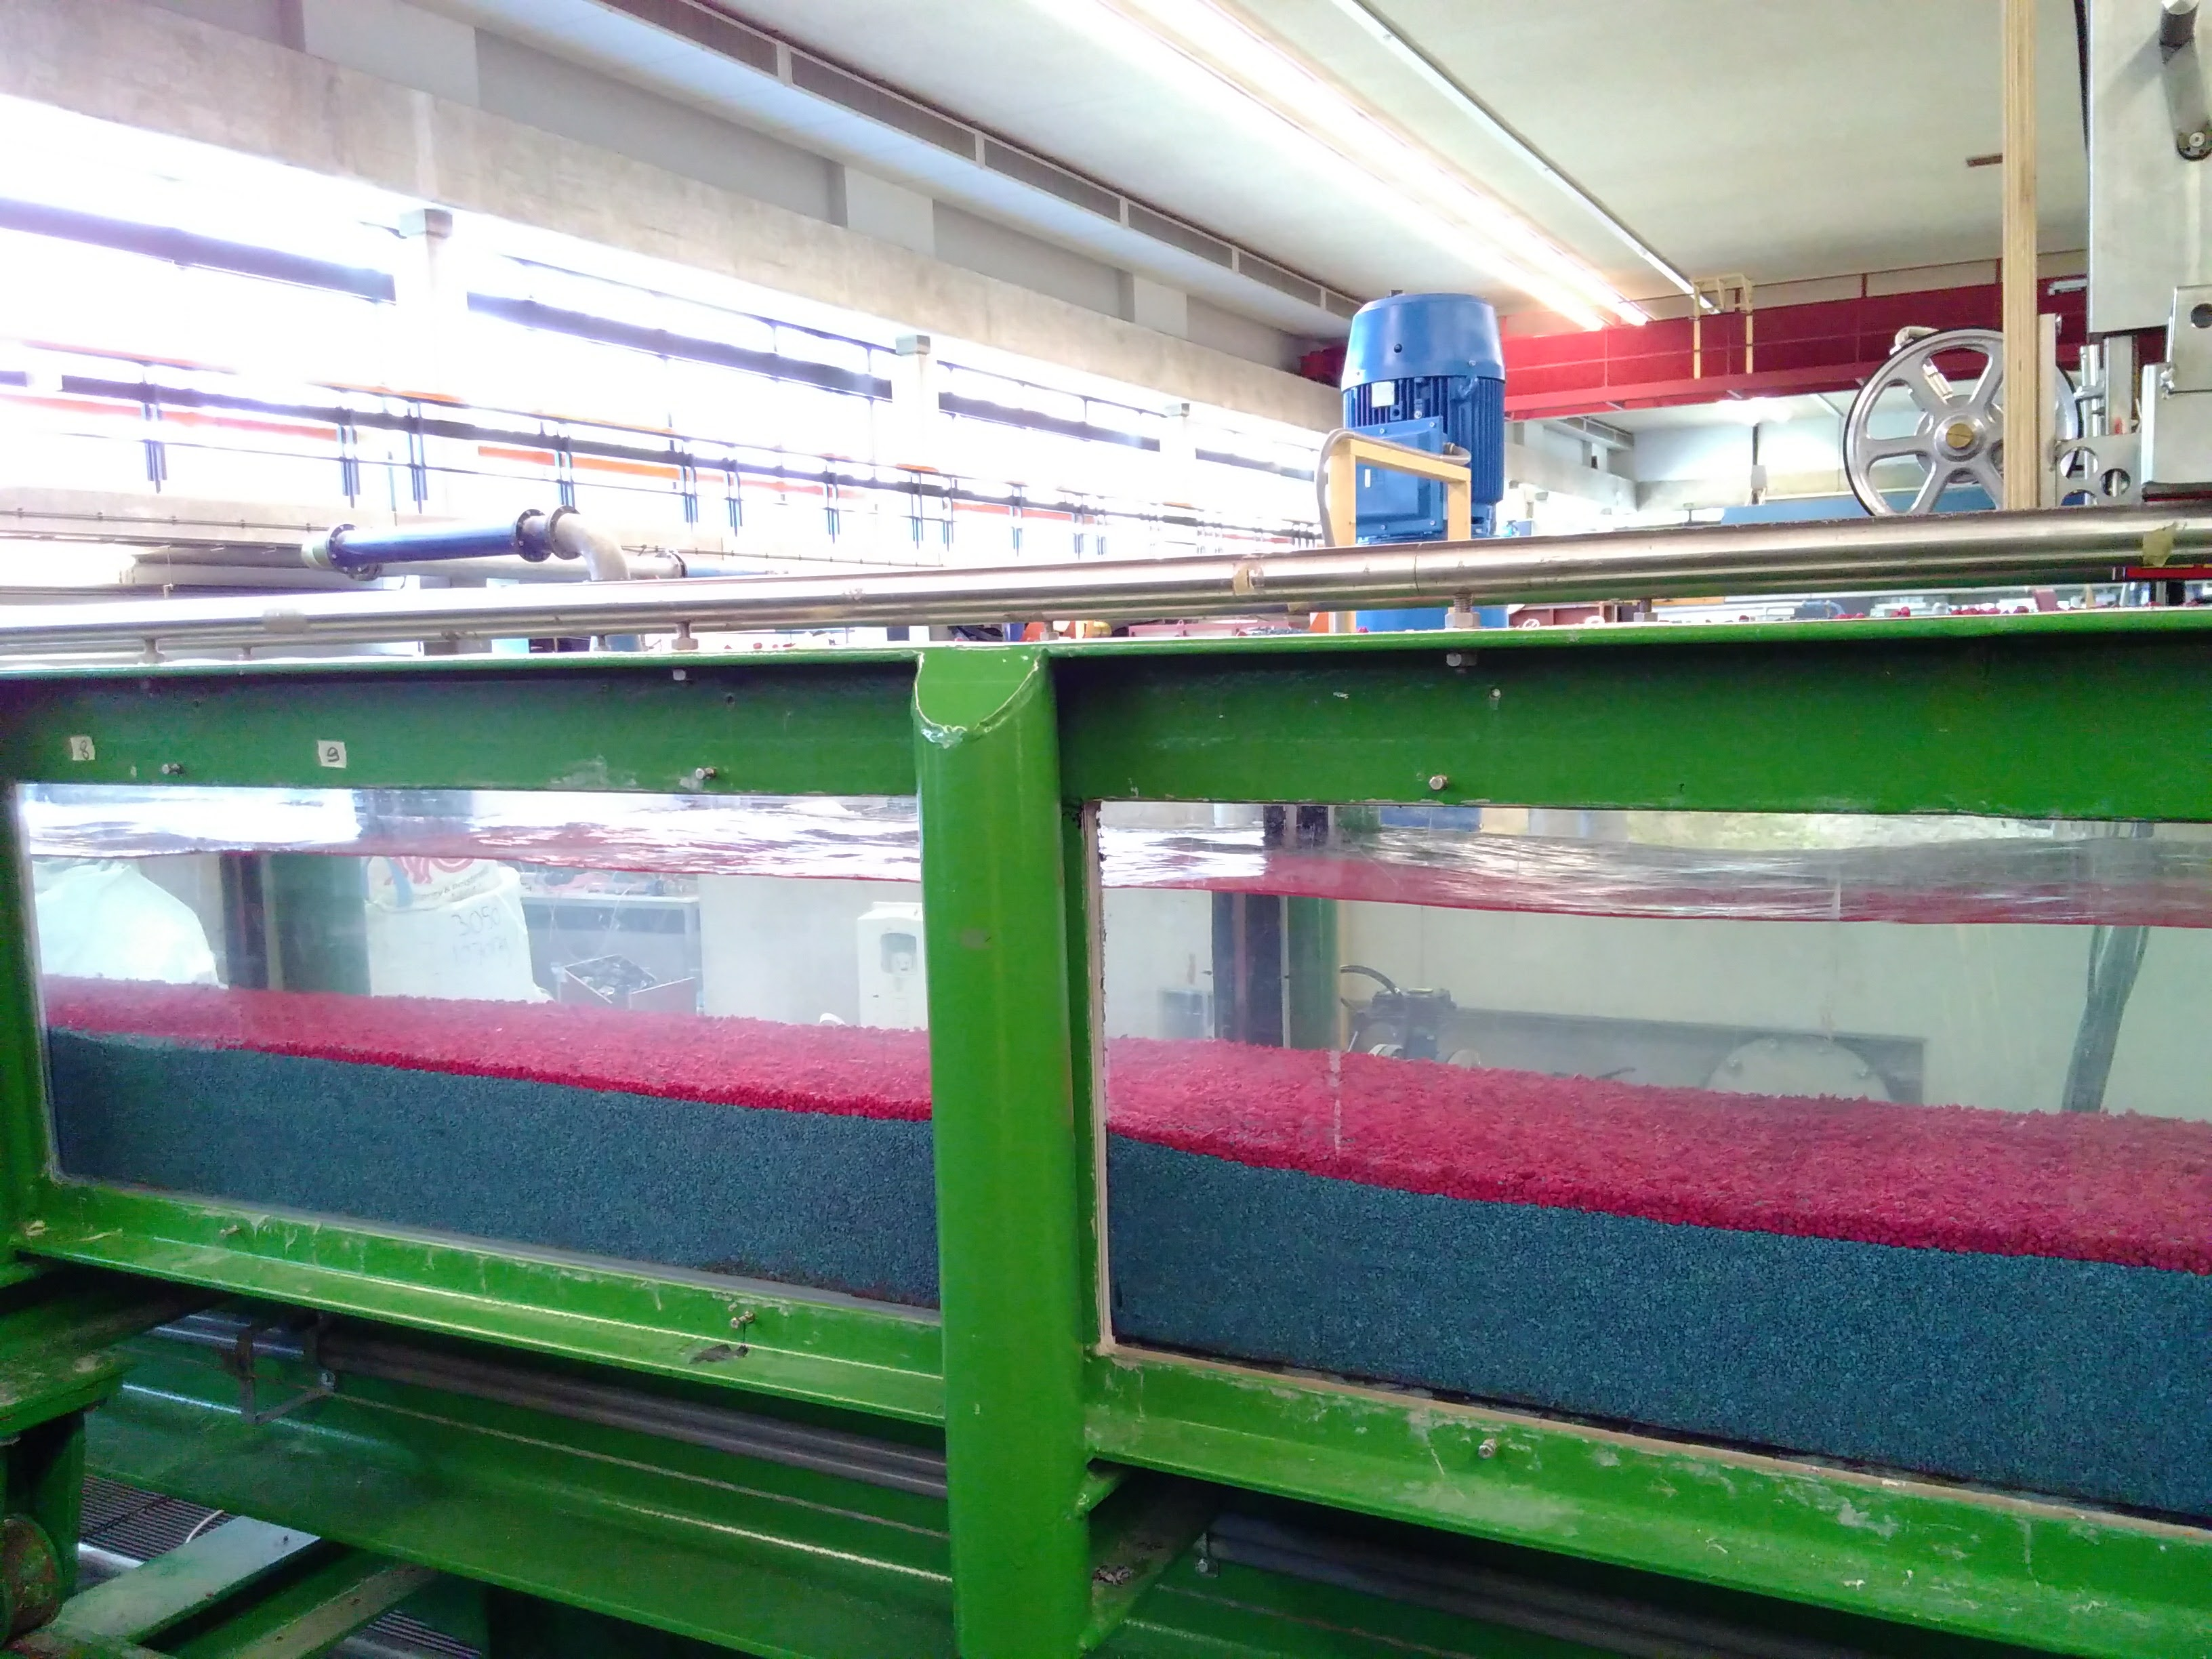
\includegraphics[height=182mm,width=182mm]{figures/cover.jpg}}

%---------references
\usepackage{natbib} %references
	\DeclareRobustCommand{\van}[3]{#2} %add \DeclareRobustCommand{\van}[3]{#3} before the bibliography

%---------math
\usepackage{array} %math arrays
\usepackage{amsmath} %math matrices
\usepackage{amssymb}
\usepackage{cancel} %cancel term in equation
\usepackage{bbm} %bold math 0 
\usepackage{bbold} %bold math characters
\usepackage{multirow} %necessary for bracket in matrix
\usepackage{bigdelim} %necessary for bracket in matrix
\usepackage{arydshln} %\hdashline[2pt/2pt] {c;{2pt/2pt}c;{2pt/2pt}c;{2pt/2pt}c}
\usepackage{upgreek} %\uppi to make \pi number and not variable

\usepackage{booktabs}

%---------include pdf
\usepackage{pdfpages} %
\usepackage{pdflscape} %\begin{landscape} \end{landscape}
%landscape
%
%\begin{landscape} 
%\includepdf[pages=-,offset=2.54cm -2.54cm,angle=0]{include/timeline.pdf}
%\end{landscape}
%portrait
%
%\includepdf[pages=-,offset=2.54cm -2.54cm]{include/CV_Erik_Mosselman.pdf}


\usepackage{graphics}
\usepackage{graphicx}
\usepackage[section]{placeins}
\graphicspath{{figures/}}
\usepackage{chngpage}

\usepackage{longtable}
%\begin{longtable}{rrp{3cm}}
%			\hline		
%			river km & date & water discharge at Lobith [\si{m^3/s}]	 \\
%			\midrule
%			\endhead
%\input{figures/adcp/measurements_overview/measurements_overview.tex} \\ %for some misterious reason, when updating the packages I needed to add this for \bottomrule not have a
%			\bottomrule
%		\caption{Summary of all ADCP profiles along the Waal River.}
%		\label{tab:table_prepos_all_all}
%\end{longtable}


%---------currency 
%use as:
%\EURO{EUR}{49500.54}
\usepackage{eurosym} 
\usepackage{euro}
\EUROSYM{EUR}{\euro}
\EUROFORMAT{main}{\out} 
\EUROFORMAT{all}{%
\form{\,}{.}{\,}%
\round{-2}%
\zero{0}{0}{}%
\plus{}{}%
\minus{\(-\)}{}
}
%
%align in table:
%\newcommand*\ALNUM{%
%\EUROFORMAT{main}{\table\out}%
%\EUROFORMAT{out}{\align\val}% % no symbol/ISO code
%\EURO{EUR}}%
%
%\begin{table}[ht]
%	\begin{center}
%	%\begin{adjustwidth}{-2cm}{-2cm}
%		\begin{tabular}{lr}		
%			\toprule
%			Fase & Coste [\euro] \\
%			\midrule
%\phaseA & \ALNUM{7000}\\
%\phaseB & \ALNUM{15000}\\
%			\bottomrule
%		\end{tabular}
%		\caption{Desglose de costes.}
%		\label{tab:costes}
%		%\end{adjustwidth}
%	\end{center}
%\end{table}
%
%different currency
%use as:
%\COP{49500.54}
%\newcommand*\COP[1]{
%{%
%\EUROFORMAT{main}{\in}%
%\EUROFORMAT{in}{\val\,COP}%
%\EUROFORMAT{EUR}{\form{\,}{.}{.}
%\round{-2}}%
%\EURO{EUR}{#1}}
%}

\usepackage{svn}
\usepackage{siunitx} %SI units

\usepackage{alphalph} %after \appendix add \renewcommand\thesection{\AlphAlph{\value{section}}} 

%figure number reset after chapter
%\usepackage{chngcntr}
%\counterwithin{figure}{chapter}

\newcommand{\addAppendix}{0} %0=no appendix; 1=add appendix
%\ifnum \addAppendix=1
%
%\fi % End of addAppendix

%general
\newcommand{\RWS}{\textit{Rijkswaterstaat~}}
\newcommand{\matlab}{Matlab\textregistered~}
\newcommand{\errmessagedisp}[1]{\errmessage{#1}\textcolor{red}{#1}}

%d3d
\newcommand{\morfac}{\textsc{MorFac}~}
\newcommand{\dtd}{Delft3D-Flow~}
\newcommand{\fm}{Delft3D-FM~}
\newcommand{\fmod}{Delft3D-FM 1D~}
\newcommand{\st}{\textsc{Sobek-3}~}
\newcommand{\waqua}{\textsc{WAQUA}~}
\newcommand{\dhydro}{D-HYDRO Suite~}
\newcommand{\sre}{\textsc{Sobek-RE}~}
\newcommand{\srur}{\textsc{Sobek-RUR}~}
\newcommand{\waqprof}{\textsc{WAQ2Prof}~}
\newcommand{\baseline}{\textsc{Baseline}~}
\newcommand{\ELV}{\textsc{ELV}}

%branches
\newcommand{\rbr}{Rhein - Boven-Rijn~}
\newcommand{\wa}{Waal~}
\newcommand{\pk}{Pannerdensh Kanaal~}
\newcommand{\nrl}{Nederrijn - Lek~}
\newcommand{\ijs}{IJssel~}
	
%math
\newcommand{\La}{L_{\mathrm{a}}}
\newcommand{\mathsub}[2]{#1_{\mathrm{#2}}}

\begin{document}
\title{\ELV}
\subtitle{One-dimensional morphodynamic research modelling}
\version{\SVN{$Revision$}}

\author{Victor Chavarrias
}
\partner{}
\coverPhoto{Frontpage: Laboratory experiment at the TU Delft modelled using \ELV.}
\date{\today}
\references{}


%authors
\authorboxi{Victor Chavarrias}
\organisationi{Deltares}

\authori{Victor Chavarrias}

\client{}
\contact{}
\keywords{}
\reference{}
\classification{}
\status{concept}
\disclaimer{}
\projectnumber{}
\documentid{}
\summary{}
%\memoTo{ELV users}
%\memoConfidentialUntil{}
%\memoDate{\today~\currenttime}
%\memoVersion{-}
%\memoFrom{
%Victor Chavarrias 
%\;\;\;\;\;\;\;\;\;\;\;\;\;\;\;\;\;\;\;\;\;\;\;\;\;\;\;\;\;\;\;\;\;\;\;\;\;\
 %Willem Ottevanger
 %}
%\memoTelephone{
%+31\,(0)88\,335\,8033 
%\;\;\;\;\;\;\;\;\;\;\;\;\;\;\;\;\;\;\;\;\;\;\;\;\;\;\;\;\;\;\;\;\;\;\;\;\;\
%+31\,(0)88\,335\,8532
%}
%\memoEmail{
%victor.chavarrias@deltares.nl 
%willem.ottevanger@deltares.nl
%}
%\memoSubject{Implementation of the Preissmann scheme in \ELV}
%\memoCopy{-}

\deltarestitle

\newpage

\chapter{Introduction}

\chapter{}
\section{Introduction}

\SVN{$Revision$}

This memo describes the implementation of the Preissmann scheme \citep{Preissmann61_2,Preissman61_3,Lyn87_2} in \ELV{} for implicitly solving the \citet{SaintVenant71} equations. 

Liselot Arkesteijn first implemented the scheme. Performance was later improved by Victor Chavarrias. 

\section{Physical system of equations}

\subsection{Set of equations}

The \citet{SaintVenant71} equations in conservative form read:
\begin{equation}
\label{eq:sv_mass}
\frac{\partial h}{\partial t}+\frac{\partial q}{\partial x}=0 \;,
\end{equation}
\begin{equation}
\label{eq:sv_mom}
\frac{\partial q}{\partial t}+\frac{\partial q^2/h}{\partial x}+\frac{1}{2}g\frac{\partial h^2}{\partial x}+gh\frac{\partial \eta}{\partial x}=-C_f\frac{q^2}{h^2} \;.
\end{equation}

The independent variables are:
\begin{itemize}
\item $x$ [\si{m}] the streamwise coordinate,
\item $t$ [\si{s}] the time coordinate.
\end{itemize}

The dependent variables are:
\begin{itemize}
\item $h$ [\si{m}] the flow depth,
\item $q$ [\si{m^2/s}] the specific discharge.
\end{itemize}

The constants are:
\begin{itemize}
\item $g$ [\si{m/s^2}] the acceleration due to gravity,
\item $\mathsub{C}{f}$ [-] the non-dimensional friction coefficient.
\end{itemize}

The constant functions of $x$ are:
\begin{itemize}
\item $\eta$ [\si{m}] the bed elevation. 
\end{itemize}

\section{Linearization of the system of equations}

We consider a reference state that is a solution to the system of equations. The reference state is a steady uniform straight flow in the $x$ direction over an inclined plane bed. Mathematically: $h_0=\text{ct.}$, $q_0=\text{ct.}$, $\frac{\partial \eta}{\partial x}=\text{ct.}=\frac{-\mathsub{C}{f}{q_0}^2}{gh_0^3}$, where ct.\ denotes a constant different from 0 and subscript $0$ indicates the reference solution. 

We add a small perturbation to the reference solution denoted by $'$ and we linearise the resulting system of equations. After substituting the reference solution we obtain a system of equations of the perturbed variables:
\begin{equation}
\label{eq:matrixf_sf}
	\frac{\partial \mathbf{G'}}{\partial t}+\mathbf{C_{0}}\frac{\partial \mathbf{G'}}{\partial x}+\mathbf{B_0}\mathbf{G'}=0 \;,
\end{equation}
where the vector of dependent variables is:
\begin{equation}
\label{eq:Q_l}
	\mathbf{G'}=\left[h',q'\right]^{\intercal} \;,
\end{equation}

The advective matrix in $x$ direction is:
\begin{equation}
\label{eq:Ax_sf}
\makebox[\textwidth][c]{$
		\mathbf{C_{0}}=\left[
 \begin{array}{cc}
%wmass 
  0 & 1  \\
%water mom x
	gh_0-\left(\frac{q_{\mathrm{x}0}}{h_0}\right)^2 & 2\frac{q_{\mathrm{x}0}}{h_0} \\
 \end{array}\right] \;.
$}
\end{equation}

The matrix of linear terms is:
\begin{equation}
\label{eq:B}
\makebox[\textwidth][c]{$
		\mathbf{B_0}=\left[
		\begin{array}{cc}
  0 & 0 \\
	\frac{-3C_{\mathrm{f}}q_{\mathrm{x}0}^2}{h_0^3} & \frac{2C_{\mathrm{f}}q_{\mathrm{x}0}}{h_0^2} \\
 \end{array}\right] \;.
$}
\end{equation}

\subsection{Boundary conditions}

The equations are solved in a one-dimensional domain of length $L$ [\si{m}] extending from $x=\mathsub{x}{o}$ until $x=\mathsub{x}{f}$ over time $T$ [\si{s}] between $t=\mathsub{t}{1}$ and $t=\mathsub{t}{2}$.

At $t=\mathsub{t}{1}$, $h=\mathsub{H}{1}(x)$ and $q=\mathsub{Q}{1}(x)$ for $\mathsub{x}{o}\leq x \leq\mathsub{x}{f}$.

At $x=\mathsub{x}{o}$, $q=\mathsub{Q}{o}(x)$ for $\mathsub{t}{1}\leq t \leq\mathsub{t}{2}$.

At $x=\mathsub{x}{f}$, $h=\mathsub{H}{f}(x)$ for $\mathsub{t}{1}\leq t \leq\mathsub{t}{2}$.

\section{Numerical discretization}

\subsection{Domain}

The space domain $x$ is discretized into $N$ cells of equal length $\Delta x$ [\si{m}]. The equations are solved at the cell centre. 

\subsection{Scheme}

The non-linear set of equations (\ref{eq:sv_mass})-(\ref{eq:sv_mom}) is discretized by means of the $\theta$-box scheme:
\begin{equation}
\frac{\partial f}{\partial t}=\frac{1}{2}\left(\frac{f_{m+1}^{n+1}-f_{m+1}^{n}}{\Delta t}+\frac{f_{m}^{n+1}-f_{m}^{n}}{\Delta t}\right) \;,
\end{equation}
\begin{equation}
\frac{\partial f}{\partial x}=\theta\left(\frac{f_{m+1}^{n+1}-f_{m}^{n+1}}{\Delta x}\right)+\left(1-\theta\right)\left(\frac{f_{m+1}^{n}-f_{m}^{n}}{\Delta x}\right) \;,
\end{equation}
where $\theta\in[0.5,1]$ is a parameter, $m\in[1,N]$ is an index indicating cell centre number in increasing order, and $n>1$ is an index indicating time. 

For $\theta=0.5$ one obtains the Preissmann scheme \citep{Preissmann61_2,Preissmann61_3,Lyn87_2}.

The first term in Equation (\ref{eq:sv_mass}) is:
\begin{equation}

\end{equation}

The slope is approximated as:
\begin{equation}
\left.\frac{\partial \eta}{\partial x}\right|_{m}=\frac{\eta_{m+1}-\eta_{m}}{\Delta x} \;,
\end{equation}



\errmessage{Jacobian terms}

\section{Solution of the algebraic system of equations}

The discretized set of equations form a system of algebraic equations:
\begin{equation}
\label{eq:alg}
\mathbf{A}\mathbf{Q}=\mathbf{B}\;.
\end{equation}

Vector:
\begin{equation}
\mathbf{Q}=[h_1, h_2, \cdots, h_{N-1}, h_N, q_1, q_2, \cdots, q_{N-1}, q_N]^{\intercal} \;,
\end{equation}
is the $2N$x1 vector of unknowns. 

Matrix:
\begin{equation}
\makebox[\textwidth][c]{$
		\mathbf{A}=\left[
		\begin{array}{cc}
  \mathbf{A}_{1} & \mathbf{A}_{2} \\
	\mathbf{A}_{3} & \mathbf{A}_{4} \\
 \end{array}\right] \;,
$} 
\end{equation}
is the $2N$x$2N$ matrix containing the implicit terms, which is subdivided into 4 $N$x$N$ submatrices contain.

Vector:
\begin{equation}
\makebox[\textwidth][c]{$
		\mathbf{B}=\left[
		\begin{array}{cc}
  \mathbf{B}_{1}\\
	\mathbf{B}_{2}\\
 \end{array}\right] \;,
$} 
\end{equation}
is the $2N$x1 vector of explicit terms. 

The system is solved using the Newton–Raphson method until $r<\epsilon$:
\begin{equation}
\label{eq:nr}
\mathbf{Q}^{j+1}=\mathbf{Q}^{j}-(\mathbf{J_0}^{j})^{-1}\left(\mathbf{A}^{j}\mathbf{Q}^{j}-\mathbf{B}^{j}\right) \;,
\end{equation}
where $j$ is the iteration index. The operation to the right of equation (\ref{eq:nr}) is done using function \texttt{mldivide} applied to arguments $\mathbf{J_0}^{j}$ and $\mathbf{A}^{j}\mathbf{Q}^{j}-\mathbf{B}^{j}$. The residual $r$ is computed as:
\begin{equation}
r=\max{\left|\left(\mathbf{A}^{j}\mathbf{Q}^{j}-\mathbf{B}^{j}\right)\right|} \;.
\end{equation}



%\begin{figure}[ht]
    %\centering
    %\includegraphics[width=\textwidth]{carraro.png}
		%\caption{Propagation of a sediment hump under steady flow condition (Figure from \citet{Carraro18_2}).}
    %\label{fig:carraro}
%\end{figure}
%
%\begin{table}[ht]
	%\begin{center}
	%\begin{adjustwidth}{-2cm}{-2cm}
		%\begin{tabular}{clcrc}		
			%\toprule
			%Case & Model & Sediment fraction(s) & Mobility & $\alpha_{\mathrm{m}}$  \\
			%\midrule
%S1 & Struiksma & fine & - &  - \\ %151
%S2 & Hirano & fine \& coarse & - & - \\ %129
%S3 & Adapted coarse layer & fine \& coarse& Shields (discrete)& 1 \\ %150
%S4 & Adapted coarse layer & fine \& coarse& Shields (continuous)& 1 \\ %153 
%S5 & Adapted coarse layer & fine \& coarse& Wilcock and McArdell (continous) & 1 \\ %154
%\midrule
%S6 & Adapted coarse layer & fine \& coarse& Shields (discrete)& 20 \\ %157
%S7 & Adapted coarse layer & 2 x fine \& coarse& Shields (discrete)& 1 \\ %158
			%\bottomrule
		%\end{tabular}
		%\caption{Simulations to model the T2 flume experiment of \citet{Struiksma99}.}
		%\label{tab:ini_diff}
		%\end{adjustwidth}
	%\end{center}
%\end{table}
%
%
%
%\section{Discussion}

%\newpage
%\appendix
%\renewcommand\thesection{\AlphAlph{\value{section}}}

%
%
%
%----------------------------
%---------BIBLIOGRAPHY
%----------------------------
%
\newpage
\section*{References}
\DeclareRobustCommand{\van}[3]{#3}
%\bibliographystyle{agufull08_mod}
\bibliography{references}

%\includepdf[pages=-]{include/timeline.pdf} 

\LastPage
\end{document}
